\chapter{Seconda istanziazione}
\section{Schema a blocchi e definizione dei segnali IN/OUT}
A partire da quanto esposto nel precedente capitolo segue lo schema di seconda istanziazione della CPU.
%\newpage
\subsection{Schema a blocchi}
\begin{figure}[H]
	\centering
	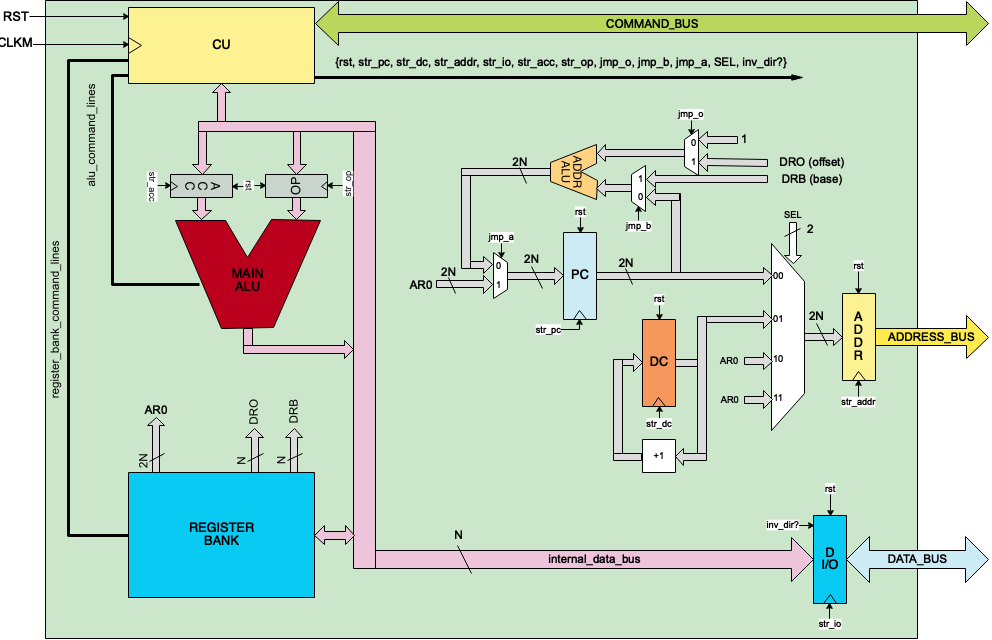
\includegraphics[scale=0.56, angle=90]{2_seconda_istanziazione}
	\label{fig:seconda_istanziazione}
\end{figure}

\newpage
\subsection{Segnali interni}
I segnali interni presenti a questo livello sono i seguenti.
\begin{itemize}
	\item \textit{rst}: \{0: funzionamento normale; 1: reset prioritario per i registri interni\}.
	\item \textit{str\_pc}: strobe per il registro PC.
	\item \textit{str\_dc}: strobe per il registro DC.
	\item \textit{str\_addr}: strobe per il registro address.
	\item \textit{str\_io}: strobe per il registro di I/O.
	\item \textit{str\_acc}: strobe per il registro accumulatore.
	\item \textit{str\_op}: strobe per il registro operando.
	\item \textit{jmp\_o}: segnale di comando per il mux. \{0: uscita = 1, 1: uscita = \textit{DRO}\}.
	\item \textit{jmp\_b}: segnale di comando per il mux. \{0: uscita = PC, 1: uscita = \textit{DRB}\}.
	\item \textit{jmp\_a}: segnale di comando per il mux. \{0: uscita = \textit{ALU\_ADDR\_OUT}, 1: uscita = \textit{AR0}\}.
	\item \textit{\textbf{SEL}}: 2 bit. Segnale di comando per il mux selezione indirizzo. Vedi \ref{2_tabella_SEL}.
	\item \textit{inv\_dir?}: \{0: registro I/O in funzionamento IN $\rightarrow$ OUT; 1: registro I/O in funzionamento OUT $\rightarrow$ IN\}.
	\item \textit{\textbf{alu\_command\_lines}}: linee di controllo per la ALU principale.
	\item \textit{\textbf{register\_bank\_command\_lines}}: linee di controllo per il register bank.
	\item \textit{\textbf{internal\_data\_lines}}: Bus dati interno a N bit.
\end{itemize}

\section{Ulteriori considerazioni di seconda istanziazione}
Per ciò che concerne l'indirizzamento della memoria si può notare che il registro indirizzo è pilotato da un mux 4-1, controllato tramite \textit{\textbf{SEL}}. \textit{\textbf{SEL}} è un segnale a 2 bit proveniente dalla CU ed il controllo del mux è schematizzato nella seguente tabella:
\begin{table}[H]
	\centering
	\footnotesize
	\fontsize{10}{18}\selectfont
	\begin{tabular}{|p{1.5cm}|p{1.5cm}|p{2.5cm}|}
		\hline
		\multicolumn{1}{|c|}{\textit{$SEL_1$}} &
		\multicolumn{1}{c|}{\textit{$SEL_0$}} & 
		\multicolumn{1}{c|}{SORGENTE ADDR}\\
		
		\hline
		\multicolumn{1}{|c|}{0} &
		\multicolumn{1}{c|}{0} & 
		\multicolumn{1}{c|}{\textbf{PC}}\\
		
		\hline
		\multicolumn{1}{|c|}{0} &
		\multicolumn{1}{c|}{1} & 
		\multicolumn{1}{c|}{\textbf{DC}}\\
		
		\hline
		\multicolumn{1}{|c|}{1} &
		\multicolumn{1}{c|}{0} & 
		\multicolumn{1}{c|}{\textbf{AR0}}\\
		
		\hline
		\multicolumn{1}{|c|}{1} &
		\multicolumn{1}{c|}{1} & 
		\multicolumn{1}{c|}{\textbf{AR0}}\\ \hline
	\end{tabular}
	\caption{Indirizzamento della memoria}
	\label{2_tabella_SEL}
\end{table}
\noindent
Questo perché, come detto, è necessario avere tre possibili sorgenti per l'indirizzamento della memoria. Il valore di indirizzamento proviene da PC, DC oppure da AR0, nei casi in cui $SEL_1$ = 1. AR0 è uno dei tre registri presenti nel banco d'appoggio con \textquotedblleft funzione speciale", ossia connesso ad un bus esterno accessibile in modo prioritario, proprio per avere la possibilità di realizzare funzioni come l'indirizzamento della memoria o il caricamento del valore del salto nel caso della jump.

\section{Dimensionamento interno dei blocchi di seconda istanziazione}
\subsection{Register bank}
\begin{figure}[H]
	\centering
	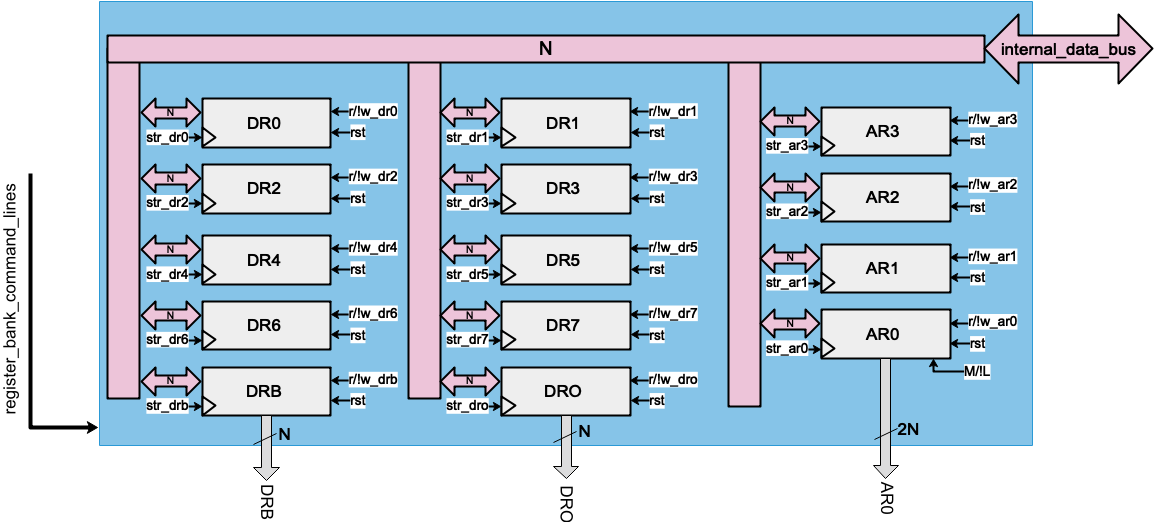
\includegraphics[scale=0.35, angle=0]{2_register_bank}
	\label{fig:register_bank}
\end{figure}
Il register bank contiene 14 registri di supporto al calcolo, di cui 4 riservati al calcolo degli indirizzi. Tra di essi vi sono tre registri accessibili esternamente attraverso altrettanti bus dedicati. Tali registri sono:
\begin{itemize}
	\item DRB: nel caso dell'operazione JBO in questo registro è presente il valore relativo alla base da sommare all'offset per il calcolo dell'indirizzo di salto.
	\item DRO: nel caso delle operazioni di JPO o JBO in questo registro è presente il valore relativo all'offset da sommare al PC o alla base per il calcolo dell'indirizzo di salto.
	\item AR0: in questo registo è presente il valore da dare al PC nel caso di jump immediata, oppure il valore da fornire alla memoria nel caso di RD o WR. Questo registro ha dimensione 2N bit per garantire l'indirizzamento a tutta la memoria, tuttavia è collegato attraverso il bus dati interno solo agli ultimi N bit. Attraverso il comando denominato $M/\overline{L}$ indirizzare il bus dati in scrittura ai primi N flip-flop o agli ultimi N flip-flop che compongono tale registro, per garantire il caricamento su tutto lo spazio dei 2N bit tramite bus a N bit. Di seguito sarà presentato lo schema interno-
\end{itemize}
Ogni registro componente il register bank è pilotato singolarmente attraverso una terna di segnali: \{\textit{str\_xxx}, \textit{rst}, \textit{r/$\overline{w}$\_xxx}\}. Nel caso del registro AR0 è presente anche il segnale $M/\overline{L}$ il cui impiego è necessario per avere la possibilità di scrivere o leggere separatemente i LSH (Least Significant Heap) o gli MSH (Most Significant Heap), ossia gli ultimi/primi N bit del registro. Dettagli del funzionamento del registro AR0 saranno esposti in seguito.\\
L'insieme dei segnali di controllo è stato schematizzato nella figura con l'insieme di linee denominato \textit{\textbf{register\_bank\_command\_lines}}.\\
Ogni registro che compone il register bank è inoltre di tipo bidirezionale a singolo bus, per avere la possibilità di essere letto o scritto attraverso il bus dati interno. Lo schema interno del generico registro, supposto N=4 bit, è rappresentato nella figura seguente.
\begin{figure}[H]
	\centering
	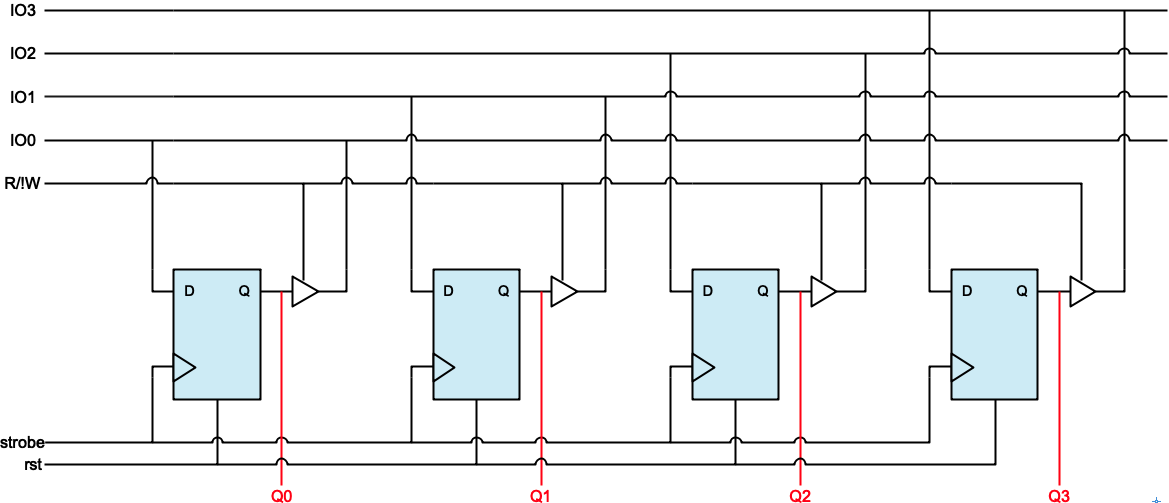
\includegraphics[scale=0.32, angle=0]{2_registro_bidir}
	\label{fig:registro_bidir}
\end{figure}
\noindent
In questo schema il comando $R/ \overline{W}$ definisce se il registro è abilitato alla lettura (1) o alla scrittura (0), in modo che il bus possa essere bidirezionale. Quando un registro non è utilizzato deve essere mantenuto in modalità scrittura ($R/ \overline{W} = 0$) per far si che i tri-state d'uscita siano disabilitati in modo da non interferire col controllo del bus da parte di altre entità ad esso collegate.
\\
In rosso invece sono rappresentate le linee d'uscita disponibili solamente per i registri con accesso speciale DRO e DRB, che costituiscono i bus dedicati discussi in precedenza.\\
Lo schema interno del registro AR0 (rappresentato per N=2 bit) è invece il seguente. Si ricorda che la dimensione di tale registro è pari a 2N bit, dunque:
\begin{figure}[H]
	\centering
	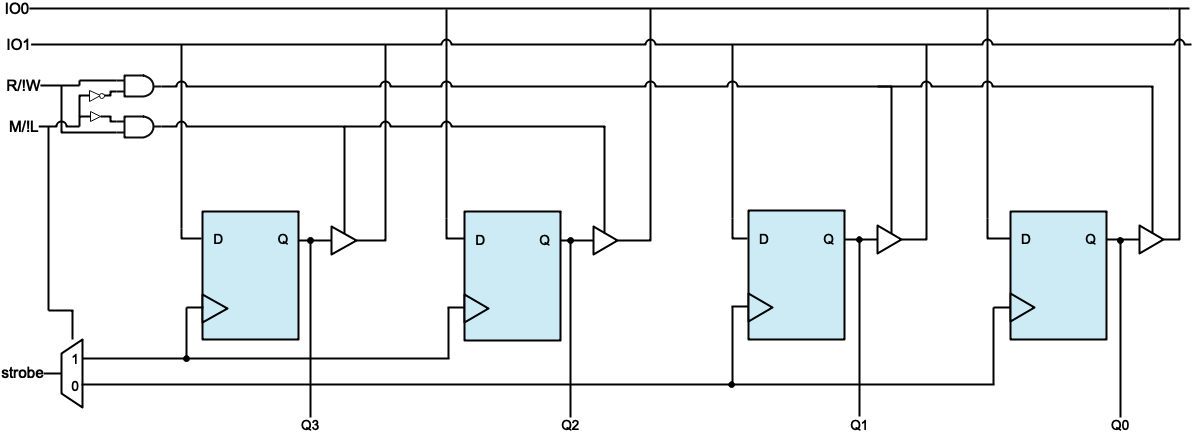
\includegraphics[scale=0.32, angle=0]{2_AR0}
	\label{fig:AR0}
\end{figure}
\noindent
Si può notare il demultiplexer interno che permette lo smistamento del segnale di strobe indipendentemente al primo o al secondo gruppo di flip-flop e la rete logica che pilota i tri-state che realizza la seguente funzione.
\begin{table}[H]
	\centering
	\fontsize{10}{18}\selectfont
	\begin{tabular}{|p{5mm}|p{5mm}|p{25mm}|}
		\hline
		\multicolumn{1}{|c|}{\textit{$R/\overline{W}$}} &
		\multicolumn{1}{c|}{\textit{$M/\overline{L}$}} & 
		\multicolumn{1}{c|}{\textbf{modalità}}\\
		
		\hline
		\multicolumn{1}{|c|}{0} &
		\multicolumn{1}{|c|}{0} & 
		\multicolumn{1}{c|}{scrittura LSH}\\
		
		\hline
		\multicolumn{1}{|c|}{0} &
		\multicolumn{1}{|c|}{1} & 
		\multicolumn{1}{c|}{scrittura MSH}\\
		
		\hline
		\multicolumn{1}{|c|}{1} &
		\multicolumn{1}{|c|}{0} & 
		\multicolumn{1}{c|}{lettura LSH}\\
		
		\hline
		\multicolumn{1}{|c|}{1} &
		\multicolumn{1}{|c|}{1} & 
		\multicolumn{1}{c|}{lettura MSH}\\ \hline
	\end{tabular}
	\caption{Modalità di funzionamento registro AR0}
\end{table}
\noindent
Omesso dal disegno, ma presente, il clear prioritario dei flip-flop connesso al segnale esterno di \textit{reset}.
\subsection{Registro IN-OUT}
Un'importante funzione è delegata al registro bidirezionale D$\_$I/O, ossia quella di pilotare il bus dati in uscita e fungere da pozzo per i dati in ingresso. Il registro deve dunque essere di tipo bidirezionale. Lo schema interno è il seguente.
\begin{figure}[H]
	\centering
	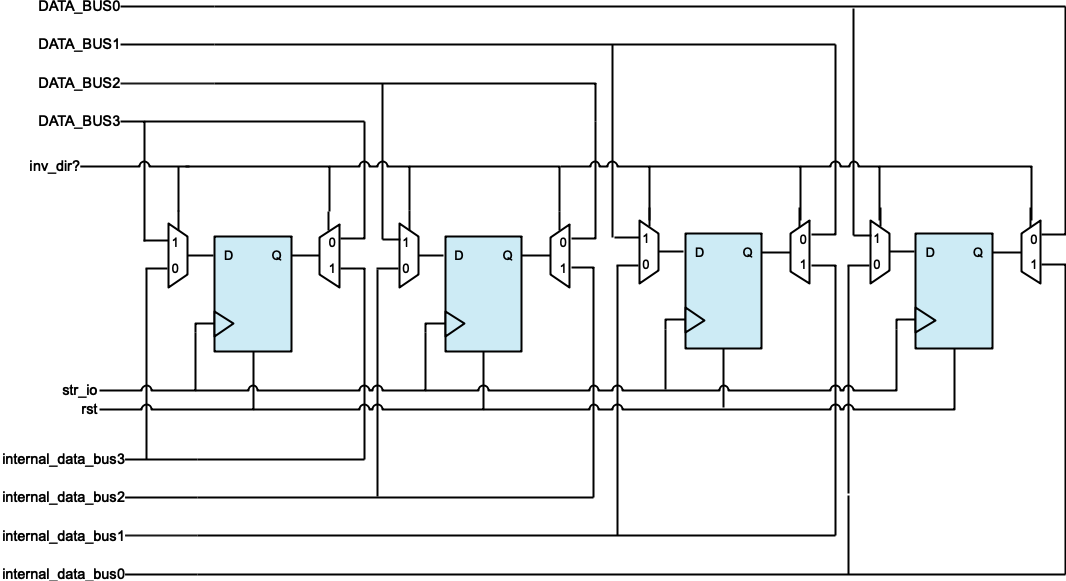
\includegraphics[scale=0.35, angle=0]{2_dio}
	\label{fig:dio}
\end{figure}
\noindent
Il registro non è dotato di buffer tri-state in ingresso/uscita, dunque sarà necessario fare in modo che questo sia sempre in modalità \textit{inv$\_$dir? = 0} quando non è in utilizzo.

\subsection{Unità di controllo: CU}
\begin{figure}[H]
	\centering
	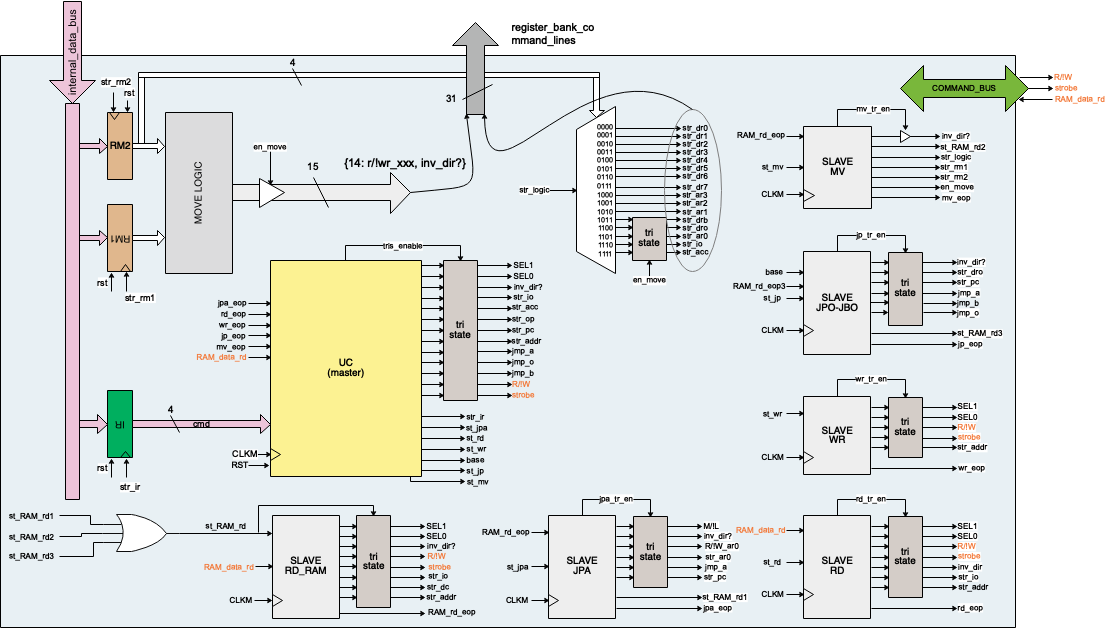
\includegraphics[scale=0.47, angle=90]{2_cu}
	\label{fig:cu}
\end{figure}
\newpage
\subsubsection{Segnali interni}
I segnali interni che trovano posto all'interno dello schema di terza istanziazione della UC sono i seguenti:
\begin{itemize}
	\item \textit{rst}: \{0: funzionamento normale; 1: reset prioritario per tutti i registri\}.
	\item \textit{str$\_$ir}: strobe per il registro istruzioni IR.
	\item \textit{\textbf{cmd}}: uscita a 4 bit dell'IR.
	\item \textit{str$\_$rm1}: strobe per il registro di supporto alla move RM1.
	\item \textit{str$\_$rm2}: strobe per il registro di supporto alla move RM2.
	\item \textit{st$\_$nomeslave}: segnale di start per lo slave \textit{nomeslave}. Delega il comando da parte della UC master allo slave \textit{nomeslave} per l'esecuzione del proprio task.
	\item \textit{nomeslave$\_$eop}: se 1 indica che lo slave \textit{nomeslave} ha terminato l'esecuzione delle proprie operazioni.
	\item \textit{base}: \{1: indica allo slave JPO/JBO se è richiesta una somma con base (JBO) prelevata dalla memoria; 0: somma JPO semplice\}\item \textit{nomeslave$\_$tr$\_$en}: lo slave \textit{nomeslave} abilita il proprio banco di buffer tri-state per pilotare le linee condivise.
	\item \textit{en$\_$move}: abilitazione dei tri-state per la logica di move.
	\item \textit{str$\_$logic}: strobe per il demux di move, esegue la copia del dato sul registro destinazione.
	\item \textit{str$\_$nomeregistro}: strobe per il registro \textit{nomeregistro}, appartenente al register bank.
	\item \textit{st$\_$RAM$\_$rdX}: segnale per lo start dello slave RD$\_$RAM. Vi sono 3 segnali provenienti da altrettanti slave che all'occorrenza abilitano RD$\_$RAM. L'abilitazione avviene tramite operazione di OR su questi tre segnali.
\end{itemize}
Inoltre, connessi al BUS COMANDI si trovano i segnali di controllo per la RAM:
\begin{itemize}
	\item \textit{R/$\overline{W}$}: \{0: abilitata scrittura della memoria RAM interna alla CPU; 1: RAM abilitata alla lettura.\}.
	\item \textit{strobe}: strobe per la memoria RAM.
	\item \textit{RAM$\_$data$\_$rd}: \{1: la RAM ha terminato la lettura o e il dato è disponibile sul BUS DATI di sistema; 0: la RAM è in stato \textit{busy}\}.
\end{itemize}

\subsubsection{Logica di Move}
Per effettuare l'operazione di move, come detto, si procede dapprima preparando i segnali che permettano lo spostamento del dato da un registro all'altro. Per fare ciò si sintetizza una logica che, a partire dalle etichette contenute in due registri di appoggio scritti a runtime, piloti i segnali da applicare ai registri sorgente e destinazione per permettere la copia del dato.
Il principio alla base della move è il fatto che tutti i registri condividono sia in lettura sia in scrittura il bus dati interno a N bit. Il bus può essere pilotato da uno dei registri coinvolti nella move (escluso ACC) attraverso l'abilitazione del segnale \textit{$r/\overline{w}\_x$} sul registro $x$. 
Si possono ora definire le etichette dei registri coinvolti nella move, come riportato nella seguente tabella.
\begin{table}[H]
	\centering
	\fontsize{10}{18}\selectfont
	\begin{tabular}{|p{25mm}|p{25mm}|p{25mm}|p{25mm}|}
		\hline
		\multicolumn{1}{|c|}{\textit{Registro}} &
		\multicolumn{1}{c|}{\textit{Etichetta}} &
		\multicolumn{1}{|c|}{\textit{Registro}} &
		\multicolumn{1}{c|}{\textit{Etichetta}}\\
		
		\hline
		\multicolumn{1}{|c|}{\textbf{DR0}} &
		\multicolumn{1}{c|}{0000} &
		\multicolumn{1}{|c|}{\textbf{DRB}} &
		\multicolumn{1}{c|}{1000}\\
		
		\hline
		\multicolumn{1}{|c|}{\textbf{DR1}} &
		\multicolumn{1}{c|}{0001} &
		\multicolumn{1}{|c|}{\textbf{DRO}} &
		\multicolumn{1}{c|}{1001}\\
		
		\hline
		\multicolumn{1}{|c|}{\textbf{DR2}} &
		\multicolumn{1}{c|}{0010} &
		\multicolumn{1}{|c|}{\textbf{AR0}} &
		\multicolumn{1}{c|}{1010}\\
		
		\hline
		\multicolumn{1}{|c|}{\textbf{DR3}} &
		\multicolumn{1}{c|}{0011} &
		\multicolumn{1}{|c|}{\textbf{AR1}} &
		\multicolumn{1}{c|}{1011}\\
		
		\hline
		\multicolumn{1}{|c|}{\textbf{DR4}} &
		\multicolumn{1}{c|}{0100} &
		\multicolumn{1}{|c|}{\textbf{AR2}} &
		\multicolumn{1}{c|}{1100}\\
		
		\hline
		\multicolumn{1}{|c|}{\textbf{DR5}} &
		\multicolumn{1}{c|}{0101} &
		\multicolumn{1}{|c|}{\textbf{AR3}} &
		\multicolumn{1}{c|}{1101}\\
		
		\hline
		\multicolumn{1}{|c|}{\textbf{DR6}} &
		\multicolumn{1}{c|}{0110} &
		\multicolumn{1}{|c|}{\textbf{ACC}} &
		\multicolumn{1}{c|}{1110}\\
		
		\hline
		\multicolumn{1}{|c|}{\textbf{DR7}} &
		\multicolumn{1}{c|}{0111} &
		\multicolumn{1}{|c|}{\textbf{D$\_$I/O}} &
		\multicolumn{1}{c|}{1111}\\
		
		\hline
	\end{tabular}
	\caption{Etichette dei registri abilitati all'operazione di move}
\end{table}
\noindent
Tali etichette possono essere definite a livello di Instruction Set, permettendo all'utente la scrittura dei registri utilizzando direttamente il nominativo nella stesura del codice assembler; es: \textit{MV DR3, ACC}.\\
La logica che pilota i segnali è di tipo combinatorio e verifica la seguente tabella di verità.
\begin{table}[H]
	\centering
	\fontsize{10}{18}\selectfont
	\begin{tabular}{|p{25mm}|p{5mm}|p{5mm}|p{25mm}|}
		\hline
		\multicolumn{1}{|c|}{\textbf{Registro sorgente}} &
		\multicolumn{1}{c|}{\textit{invDir?}} &
		\multicolumn{1}{|c|}{\textit{M/$\overline{L}$}} &
		\multicolumn{1}{c|}{\textit{R/$\overline{W}$}}\\
		
		\hline
		\multicolumn{1}{|c|}{\textbf{DR0}} &
		\multicolumn{1}{c|}{-} &
		\multicolumn{1}{|c|}{-} &
		\multicolumn{1}{c|}{DR0}\\
		
		\hline
		\multicolumn{1}{|c|}{\textbf{DR1}} &
		\multicolumn{1}{c|}{-} &
		\multicolumn{1}{|c|}{-} &
		\multicolumn{1}{c|}{DR1}\\
		
		\hline
		\multicolumn{1}{|c|}{\textbf{DR2}} &
		\multicolumn{1}{c|}{-} &
		\multicolumn{1}{|c|}{-} &
		\multicolumn{1}{c|}{DR2}\\
		
		\hline
		\multicolumn{1}{|c|}{\textbf{DR3}} &
		\multicolumn{1}{c|}{-} &
		\multicolumn{1}{|c|}{-} &
		\multicolumn{1}{c|}{DR3}\\
		
		\hline
		\multicolumn{1}{|c|}{\textbf{DR4}} &
		\multicolumn{1}{c|}{-} &
		\multicolumn{1}{|c|}{-} &
		\multicolumn{1}{c|}{DR4}\\
		
		\hline
		\multicolumn{1}{|c|}{\textbf{DR5}} &
		\multicolumn{1}{c|}{-} &
		\multicolumn{1}{|c|}{-} &
		\multicolumn{1}{c|}{DR5}\\
		
		\hline
		\multicolumn{1}{|c|}{\textbf{DR6}} &
		\multicolumn{1}{c|}{-} &
		\multicolumn{1}{|c|}{-} &
		\multicolumn{1}{c|}{DR6}\\
		
		\hline
		\multicolumn{1}{|c|}{\textbf{DR7}} &
		\multicolumn{1}{c|}{-} &
		\multicolumn{1}{|c|}{-} &
		\multicolumn{1}{c|}{DR7}\\
		
		\hline
		\multicolumn{1}{|c|}{\textbf{DRB}} &
		\multicolumn{1}{c|}{-} &
		\multicolumn{1}{|c|}{-} &
		\multicolumn{1}{c|}{DRB}\\
		
		\hline
		\multicolumn{1}{|c|}{\textbf{DRO}} &
		\multicolumn{1}{c|}{-} &
		\multicolumn{1}{|c|}{-} &
		\multicolumn{1}{c|}{DRO}\\
		
		\hline
		\multicolumn{1}{|c|}{\textbf{AR0}} &
		\multicolumn{1}{c|}{-} &
		\multicolumn{1}{|c|}{0} &
		\multicolumn{1}{c|}{AR0}\\
		
		\hline
		\multicolumn{1}{|c|}{\textbf{AR1}} &
		\multicolumn{1}{c|}{-} &
		\multicolumn{1}{|c|}{-} &
		\multicolumn{1}{c|}{AR1}\\
		
		\hline
		\multicolumn{1}{|c|}{\textbf{AR2}} &
		\multicolumn{1}{c|}{-} &
		\multicolumn{1}{|c|}{-} &
		\multicolumn{1}{c|}{AR2}\\
		
		\hline
		\multicolumn{1}{|c|}{\textbf{AR3}} &
		\multicolumn{1}{c|}{-} &
		\multicolumn{1}{|c|}{-} &
		\multicolumn{1}{c|}{AR3}\\
		
		\hline
		\multicolumn{1}{|c|}{\textbf{ACC}} &
		\multicolumn{1}{c|}{-} &
		\multicolumn{1}{|c|}{-} &
		\multicolumn{1}{c|}{-}\\
		
		\hline
		\multicolumn{1}{|c|}{\textbf{D$\_$I/O}} &
		\multicolumn{1}{c|}{0} &
		\multicolumn{1}{|c|}{-} &
		\multicolumn{1}{c|}{-}\\
		\hline
	\end{tabular}
	\caption{Tabella di verità per la sintesi della logica di move}
\end{table}
\noindent
La lettura della tabella avviene come segue: per ogni registro scelto i segnali da abilitare sono quelli aventi un valore valido nella tabella.\\
Per esempio, per usare il registro \textbf{AR0} come sorgente la logica deve generare i segnali \textit{M/$\overline{L}$ = 0} e \textit{R/$\overline{W}\_$AR0 = 1} ponendo tutti gli altri a 0, mentre se si scegliesse \textbf{D$\_$I/O} la logica genererebbe solamente \textit{inv$\_$dir? = 0}. Le uscite sono dunque 16 e sono abilitate tramite buffer tri-state da parte di un segnale di controllo \textit{en$\_$move}.
\par \bigskip \noindent
Passiamo ora a definire i diagrammi ASM per le MSF slave interne alla UC.
\newpage
\subsubsection{Slave RD$\_$RAM}
Esegue la lettura della memoria di un dato indirizzando la RAM tramite il DC. Il diagramma ASM è il seguente.
\begin{figure}[H]
	\centering
	\includegraphics[scale=0.5]{ASM_ram_rd}
	\label{fig:asm_ram_rd}
\end{figure}

\newpage
\subsubsection{Slave JPA}
Esegue la jump immediata, aggiornando il Program Counter all'indirizzo di salto ricavato dalla memoria.
\begin{figure}[H]
	\centering
	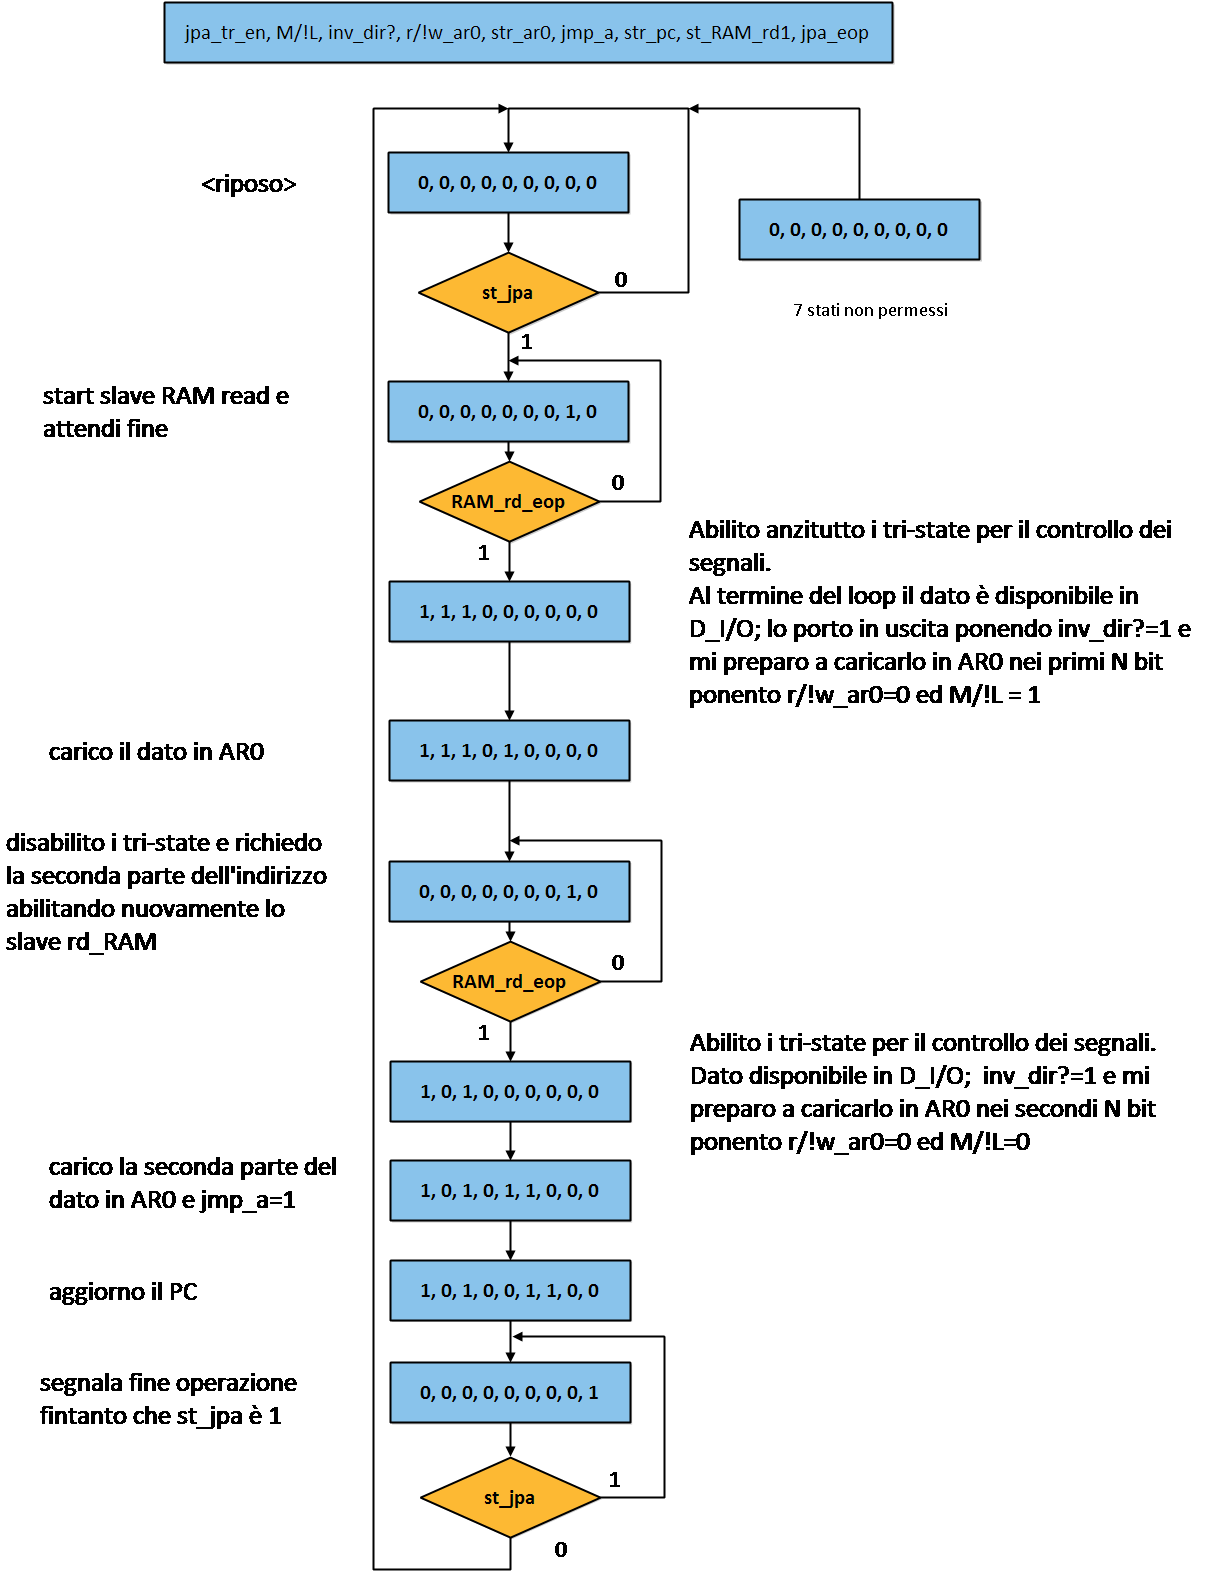
\includegraphics[scale=0.43]{asm_jpa}
	\label{fig:asm_jpa}
\end{figure}

\newpage
\subsubsection{Slave RD}
Esegue la lettura della memoria all'indirizzo presente in AR0 e salva il dato sul registro D$\_$I/O.
\begin{figure}[H]
	\centering
	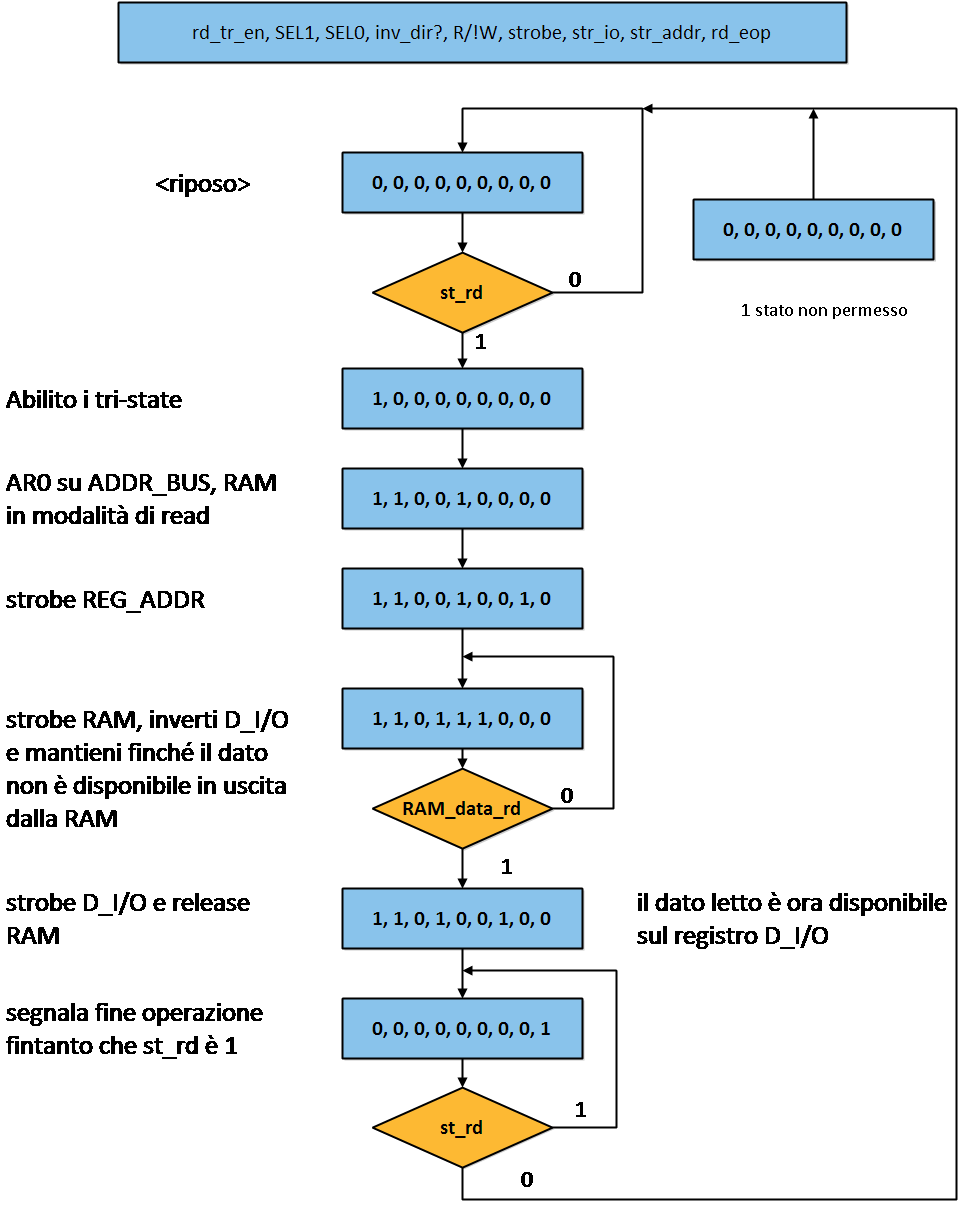
\includegraphics[scale=0.55]{asm_rd}
	\label{fig:asm_rd}
\end{figure}

\newpage
\subsubsection{Slave WR}
Esegue la scrittura del dato presente in D$\_$I/O nella memoria alla locazione imposta dall'indirizzo presente in AR0.
\begin{figure}[H]
\centering
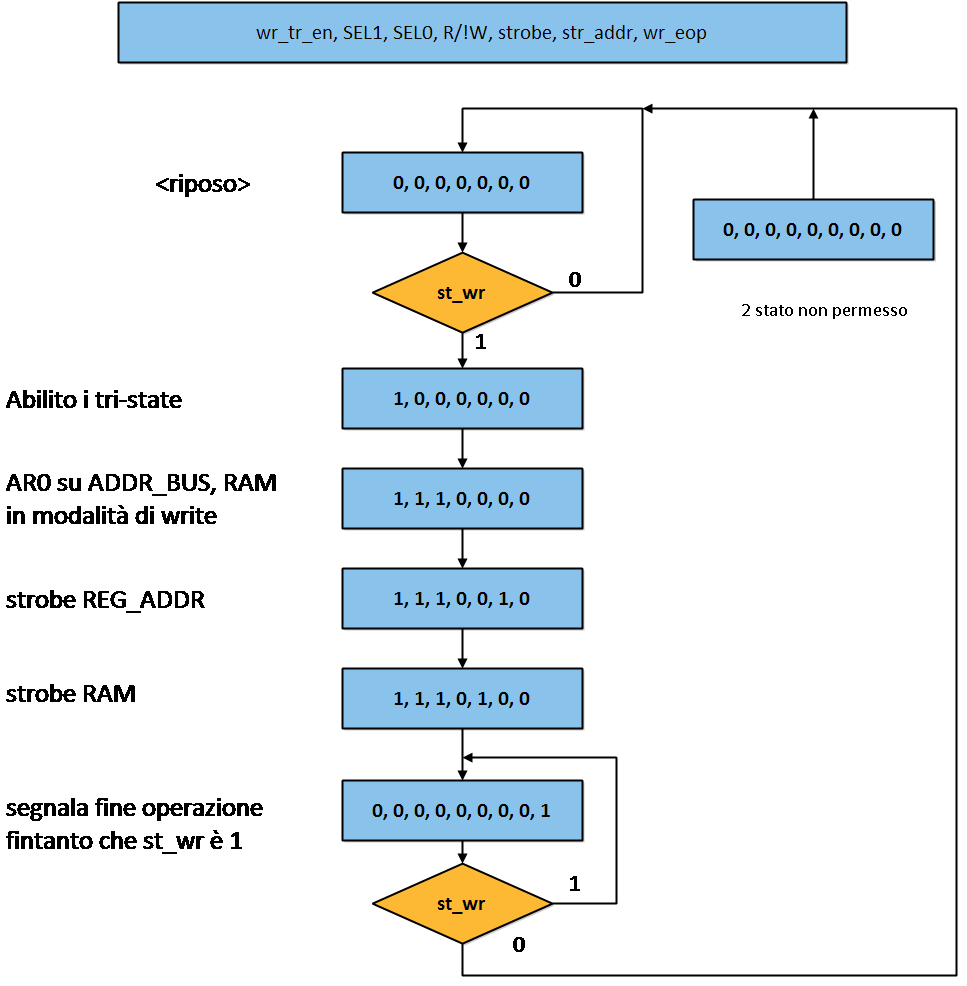
\includegraphics[scale=0.55]{asm_wr}
\label{fig:asm_wr}
\end{figure}

\newpage
\subsubsection{Slave JPO$\_$JBO}
Esegue la jump all'indirizzo dato dalla somma di una \textit{base} e un offset. Mentre l'offset proviene dalla memoria, la base può essere l'indirizzo corrente del PC o un ulteriore dato prelevato dalla memoria.
\begin{figure}[H]
	\centering
	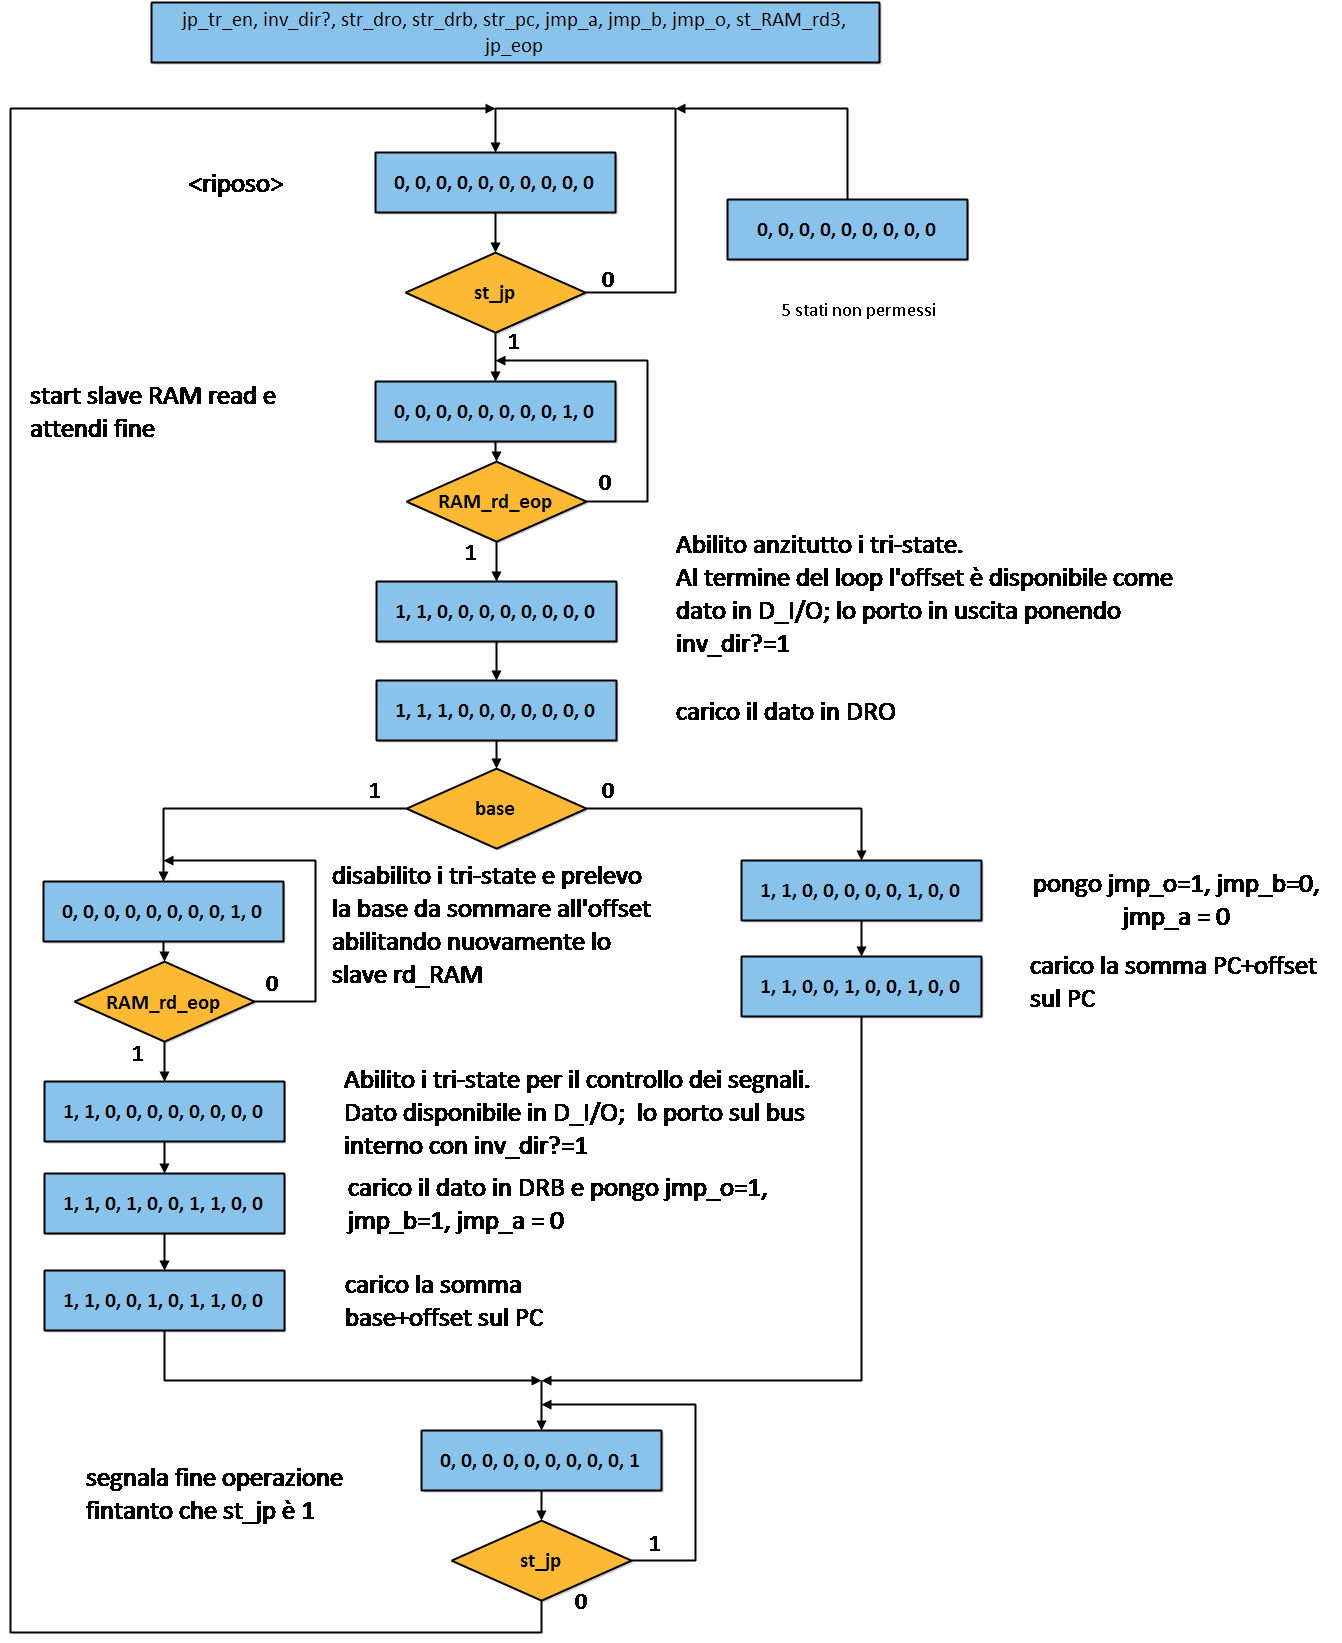
\includegraphics[scale=0.40]{asm_jp}
	\label{fig:asm_jp}
\end{figure}

\newpage
\subsubsection{Slave MV}
Esegue la copia del dato da un registro sorgente ad uno destinazione indirizzati tramite etichetta prelevata dalla memoria.
\begin{figure}[H]
	\centering
	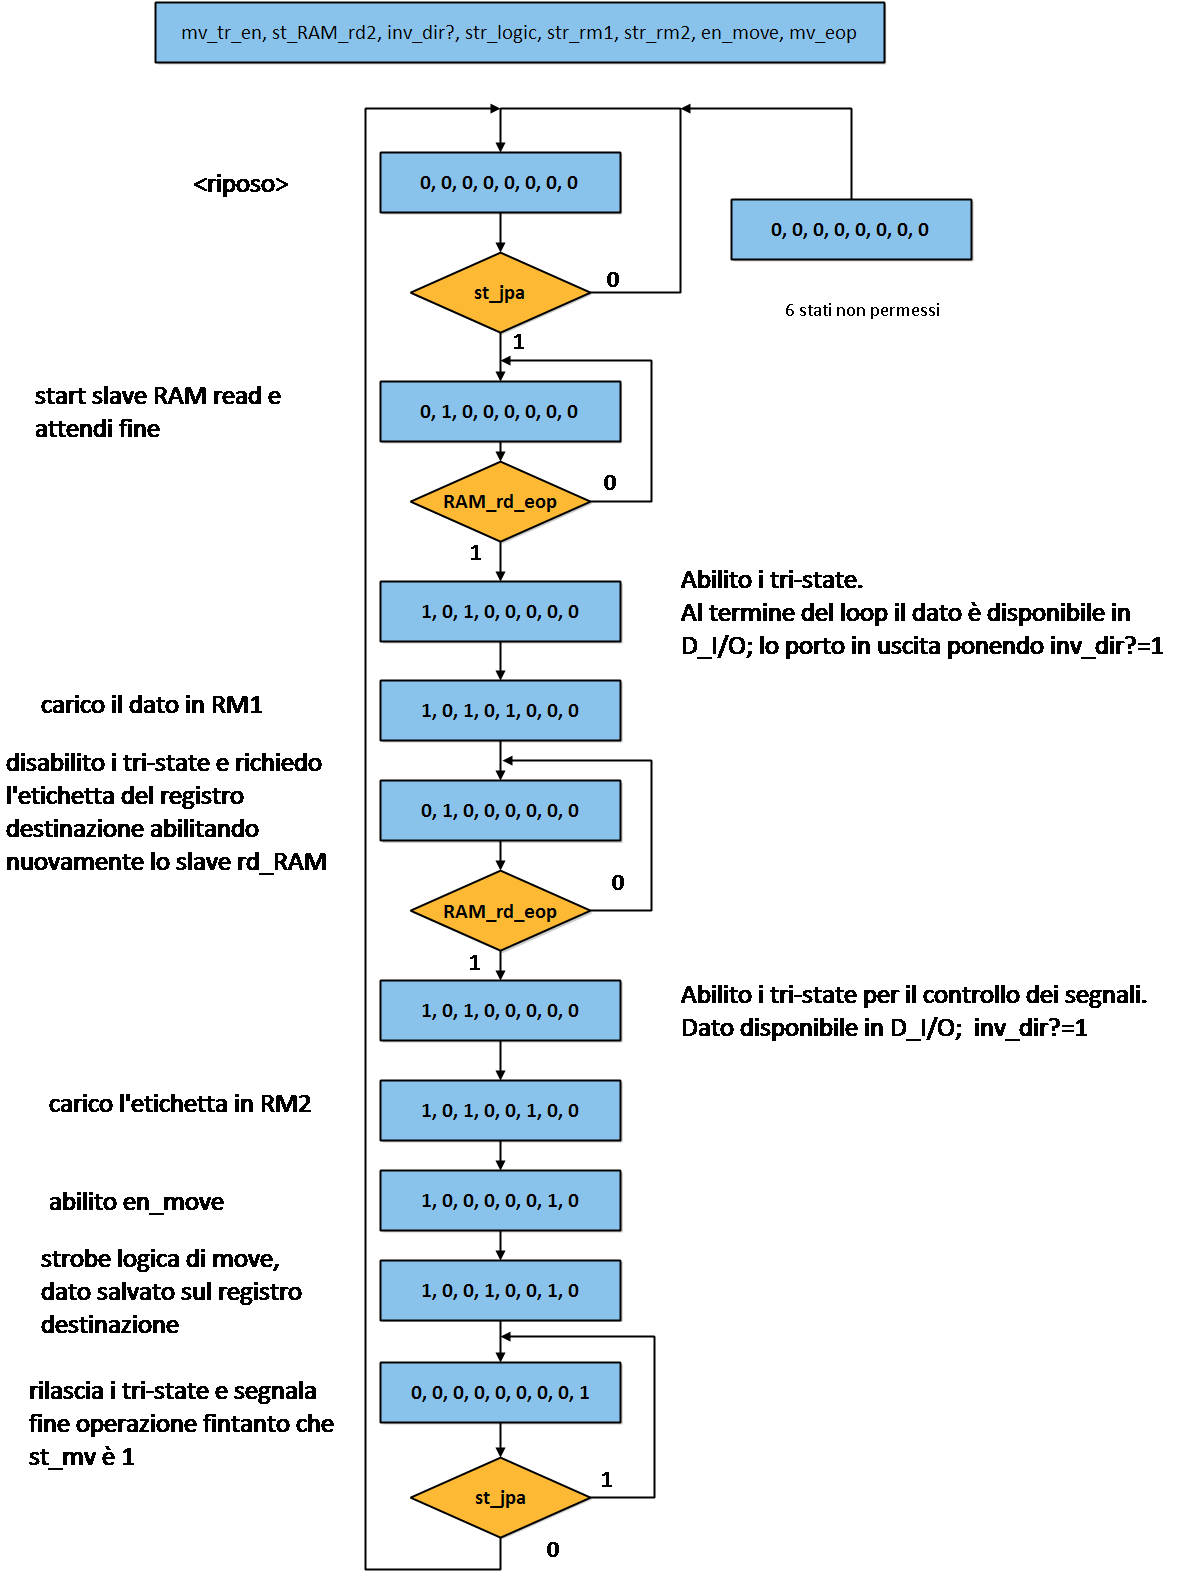
\includegraphics[scale=0.43]{asm_mv}
	\label{fig:asm_mv}
\end{figure}

\newpage
\subsubsection{ASM MASTER}
Infine, il diagramma ASM per la macchina master che esegue le fasi di fetch e decode, delegando l'execute agli slave. Le azioni da svolgere sono:\\
\par \bigskip \noindent
FETCH:
\begin{enumerate}
	\item Poni PC su ADDR$\_$BUS, RAM in modalità di read.
	\item Strobe REG$\_$ADDR
	\item RIPETI: Strobe RAM e poni inv$\_$dir=1 FINCHÉ RAM$\_$data$\_$rd = 1
	\item Strobe IR e incrementa PC
\end{enumerate}

\par \bigskip \noindent
DECODE:
\begin{enumerate}
	\item L'uscita del registro istruzioni IR contiene il codice relativo all'istruzione da eseguire. Una serie di controlli interni identifica l'operazione definita dai segnali di \textbf{\textit{cmd}}.
\end{enumerate}

\par \bigskip \noindent
EXECUTE (WRITE-BACK):
\begin{enumerate}
	\item Riconosciuta l'istruzione la macchina MASTER delega il controllo dell'hardware interno allo slave che eseguirà l'istruzione e cederà nuovamente il controllo alla master. Lo slave si occupa anche di un eventuale WRITE-BACK in memoria.
\end{enumerate}

\noindent
Da cui il diagramma ASM per la macchina MASTER.
\begin{figure}[H]
	\centering
	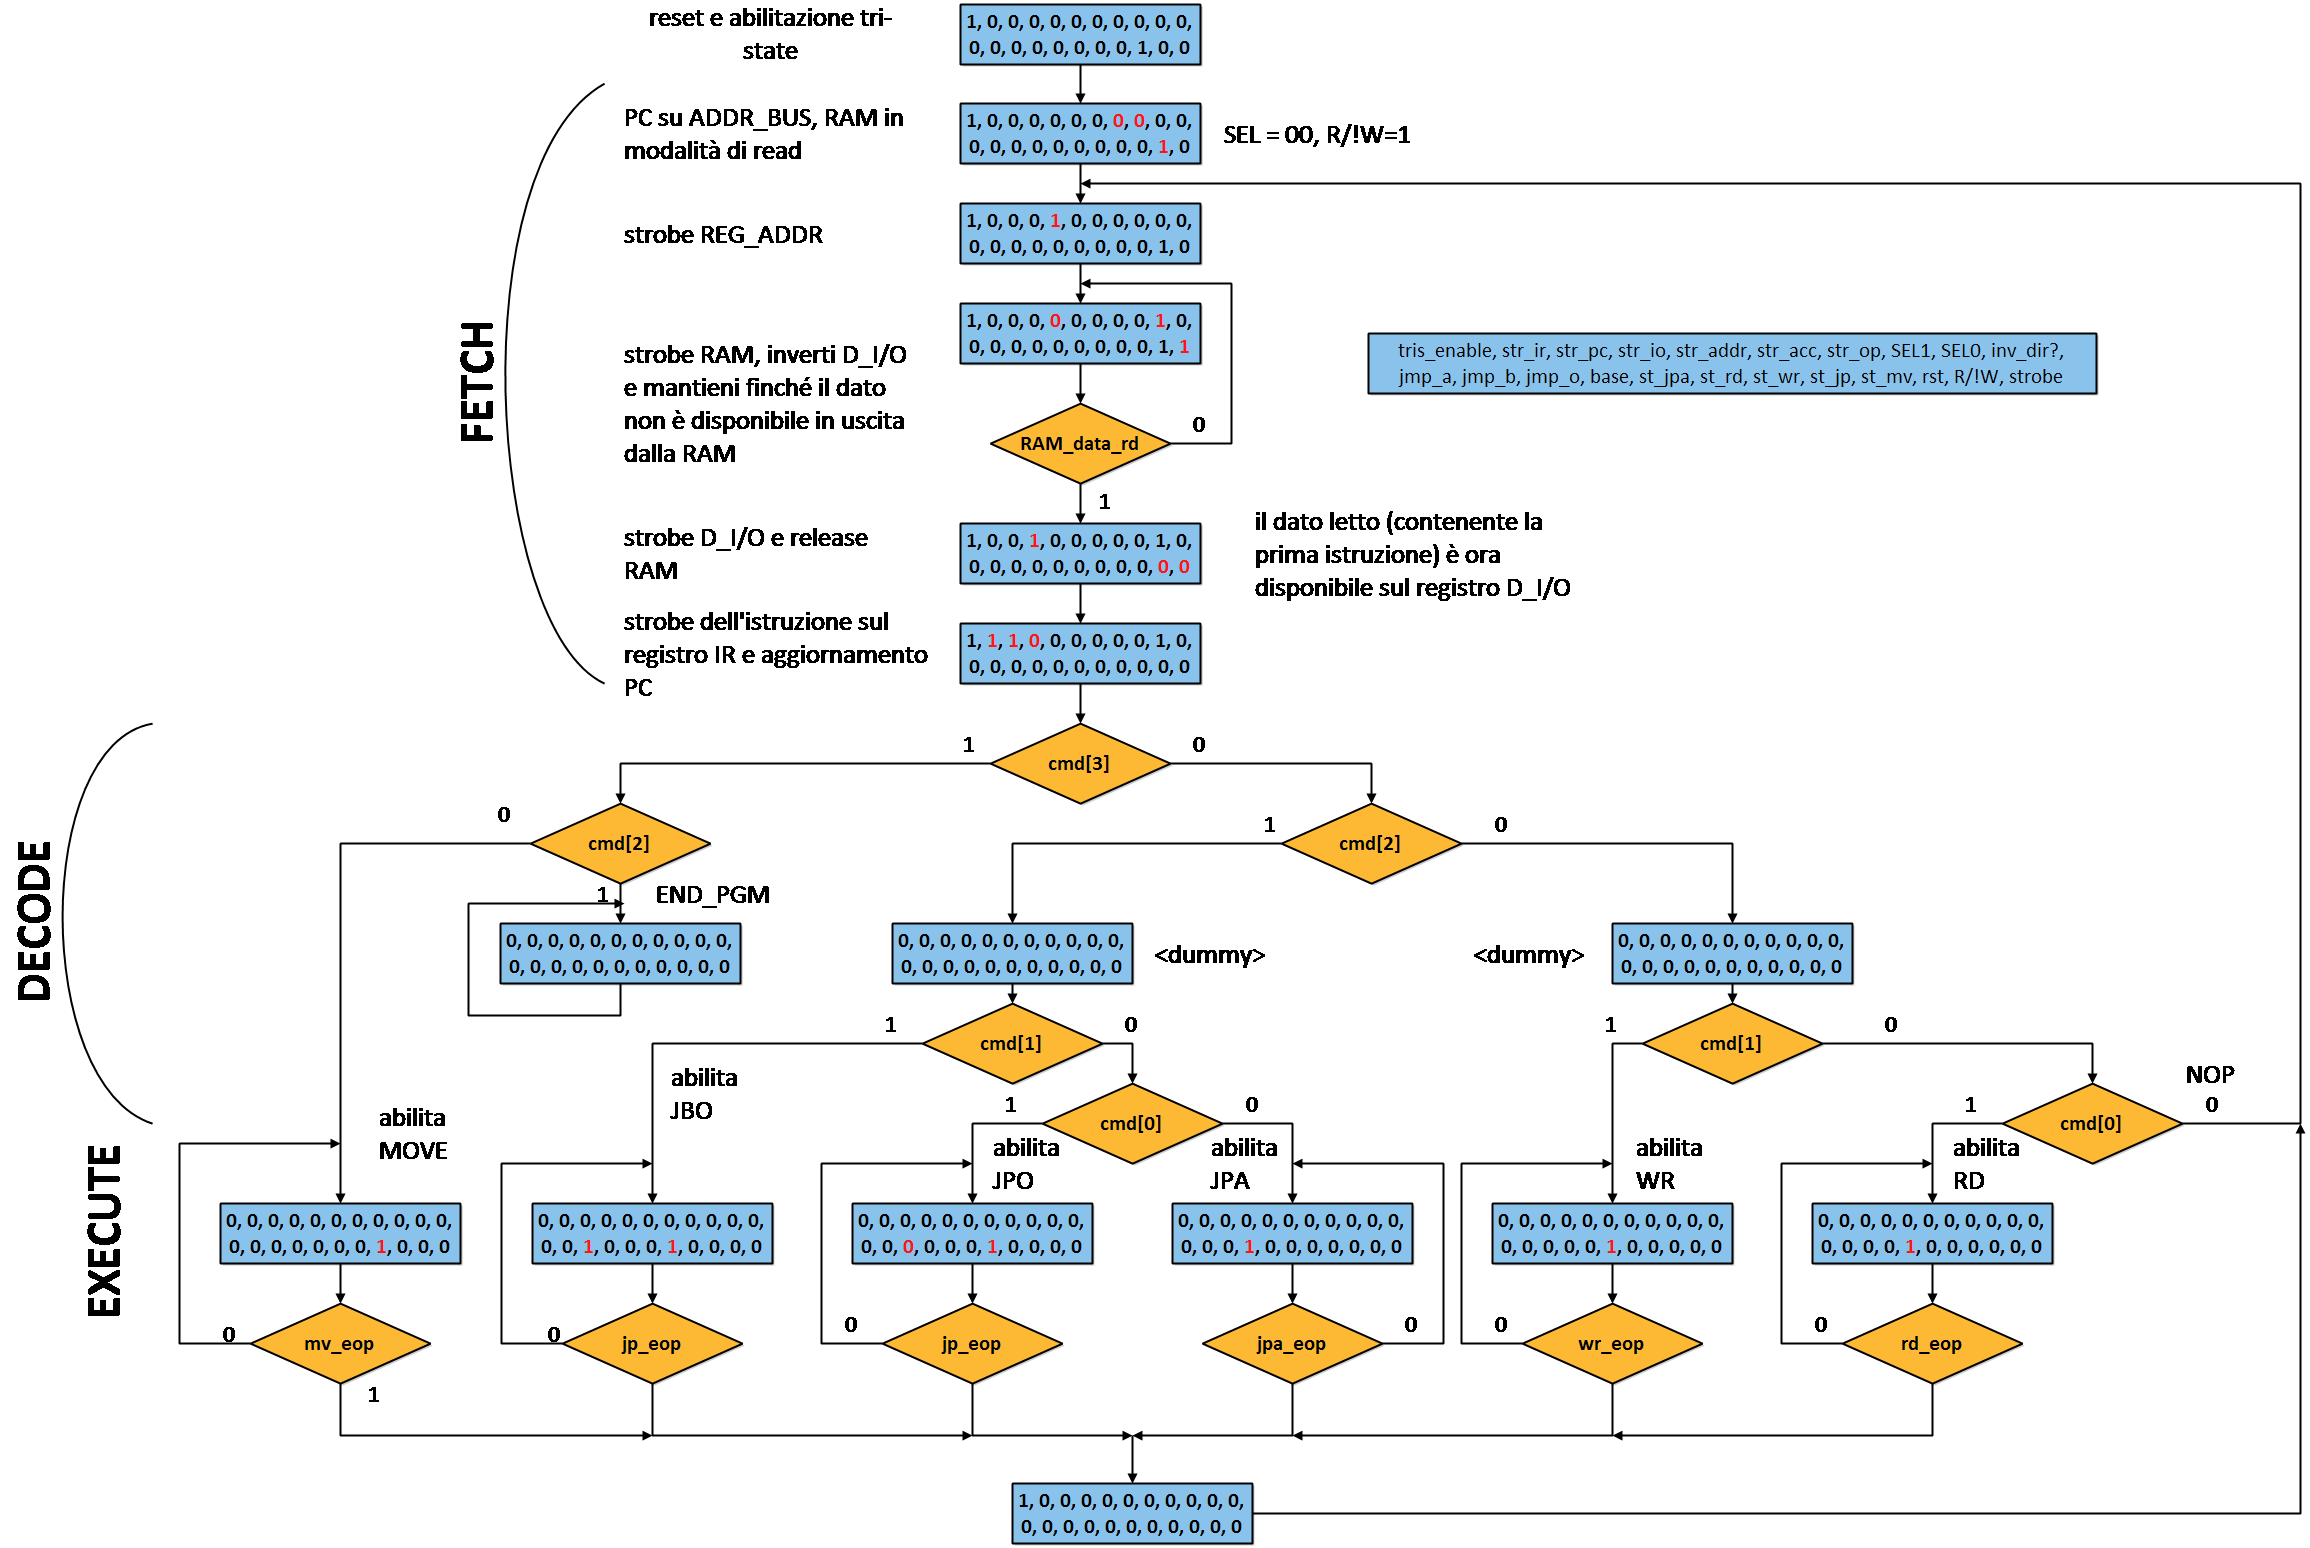
\includegraphics[scale=0.35, angle=90]{asm_master}
	\label{fig:asm_master}
\end{figure}

